\documentclass[thesis.tex]{subfiles}
\begin{document}

\chapter{Related Work}
\label{chap:prevwork}

% Categories from GISTAR
% * Finite Elements (also contains voxel based GI)
% * Monte-Carlo ray tracing
% * Photon Mapping
% * Instant Radiosity
% * Many lights (hierarchical! gathering of lights)
% * Point-based (render points somehow)
% * Discrete ordinate methods (propagation volumes etc.)
% * Precomputation

This chapter gives an overview of related realtime global illumination techniques.
Ritschel et al. \cite{bib:RealtimeGIOverview} already gave a great overview over this field for all approaches before 2012.
Therefore, we will focus on newer methods and those which are either fundamental, similar or inspirational to this thesis instead of trying to cover the whole field.

\section {Many-Lights Methods}
\begin{figure}[h]
	\centering
	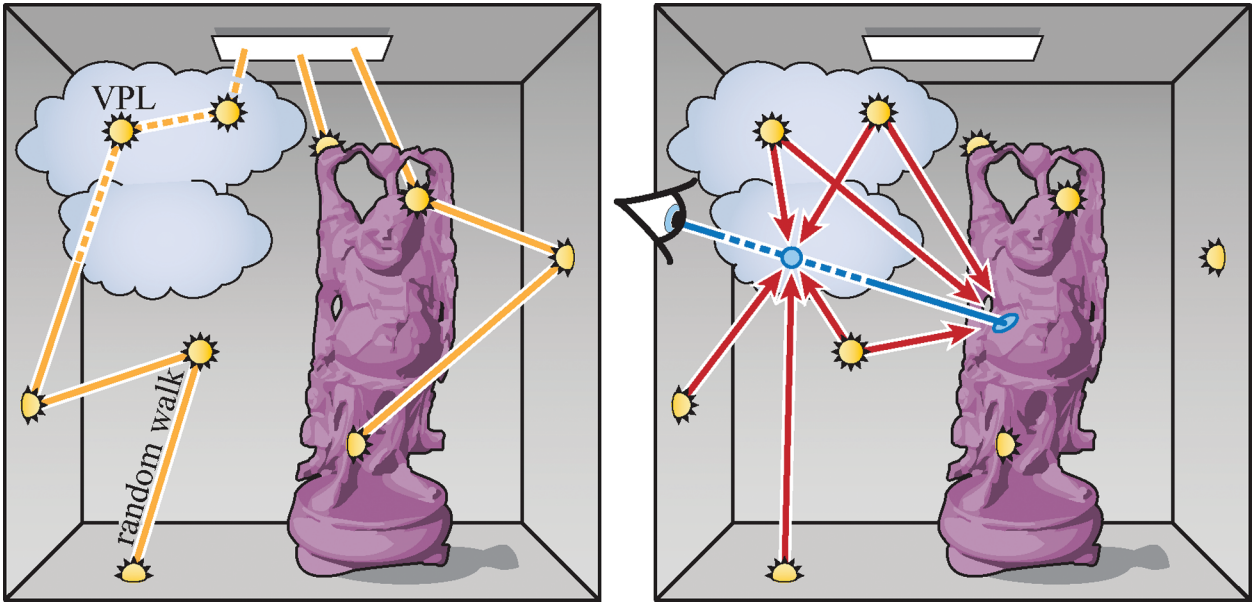
\includegraphics[width=0.8\textwidth]{manylights}
	\caption{\cite{bib:manylightssurvey2014} Two passes of many-light algorithms: Left distribution of virtual lights, right direct lighting using virtual lights.} \label{fig:manylights}
\end{figure}
Many-light methods reduce the global illumination to the smaller problem of calculating the direct lighting of many virtual light sources.
All many-light approaches perform two passes (see \autoref{fig:manylights}):
First virtual light sources are distributed in the scene, second each virtual light source performs direct lighting.
The main advantages of the many-light approach in general is its relatively easy unified framework and its good scalability in performance and quality.
Global illumination using $M$ virtual point lights can generally be expressed as following:
\begin{equation}
L_o(\mathrm{x}, \omega_o) = \sum\limits_{i=1}^{M} f_r(\mathrm{x}, \overrightarrow{\mathrm{x}\mathrm{x}_i}, \omega_o) \cdot G(\mathrm{x}, \mathrm{x}_i) \cdot V(\mathrm{x}, \mathrm{x}_i) \cdot f_r(\mathrm{x}_i, \omega_i, \overrightarrow{\mathrm{x}_i\mathrm{x}}) \cdot \phi_i
\end{equation}
Where $G(\mathrm{x}, \mathrm{x}_i)$ is the geometry term which describes the light transfer from the virtual light in $x_i$ to the surface in point $x$.
It depends on the type of the virtual light source.
$V(\mathrm{x}, \mathrm{x}_i)$ is the visibility of a virtual light and $\phi_i$ its incoming flux.

Dachsbacher et al. \cite{bib:manylightssurvey2014} did recently a detailed survey on many-lights for both offline and real-time rendering.
We focus here on the most important real-time approaches.

\subsection{Reflective Shadow Mapping}
One of the most important real-time global illumination algorithms is reflective shadow mapping by Dachsbacher et al. \cite{bib:reflectiveshadowmaps} on which many other approaches, including the one presented in this thesis, rely.
It handles the virtual light distribution with the rasterization of an extended shadow map, the reflective shadow map (RSM).
The RSM does not only contain depth as normal shadow maps, but also the reflected flux and the normal of the surface in each texel.
Each texel of this shadow map is then seen as virtual point light (VPL).
The original paper shades each pixel with a given number of sampled VPLs without taking indirect shadows into account.
Also, the technique handles only a single indirect bounce of diffuse lighting which means that a VPL is strictly speaking a hemispherical lambert emitter.
(However, as most literature we will use the term "VPL" interchangable)

\todo{clustering stuff}

\subsection{VPL Bias and Compensation}
Using virtual point lights, the geometry term is defined as following:
\begin{align}
G(\mathrm{x}, \mathrm{x}_i) = \frac{(\hat{\mathbf{n}} \cdot \overrightarrow{\mathrm{x}\mathrm{x}_i} )^+}{||\mathrm{x} - \mathrm{x}_i||^2} \cdot (\hat{\mathbf{n}}_i \cdot \overrightarrow{\mathrm{x}_i\mathrm{x}})^+
\end{align}
Where $\mathbf{n}$ and $\mathbf{n}_i$ are the surface normals in point $\mathrm{x}$ and $\mathrm{x}_i$ respectively.
Note that the geometry term is a combination of the photometric distance law (fraction of cosine of angle to light source and squared distance to light source) and the definition of intensity for Lambert emitter (cosine of angle to receiver) as described earlier in \autoref{sec:preq:theo:relation}.
\\
\begin{figure}[h]
\centering
\begin{subfigure}[b]{0.48\textwidth}
	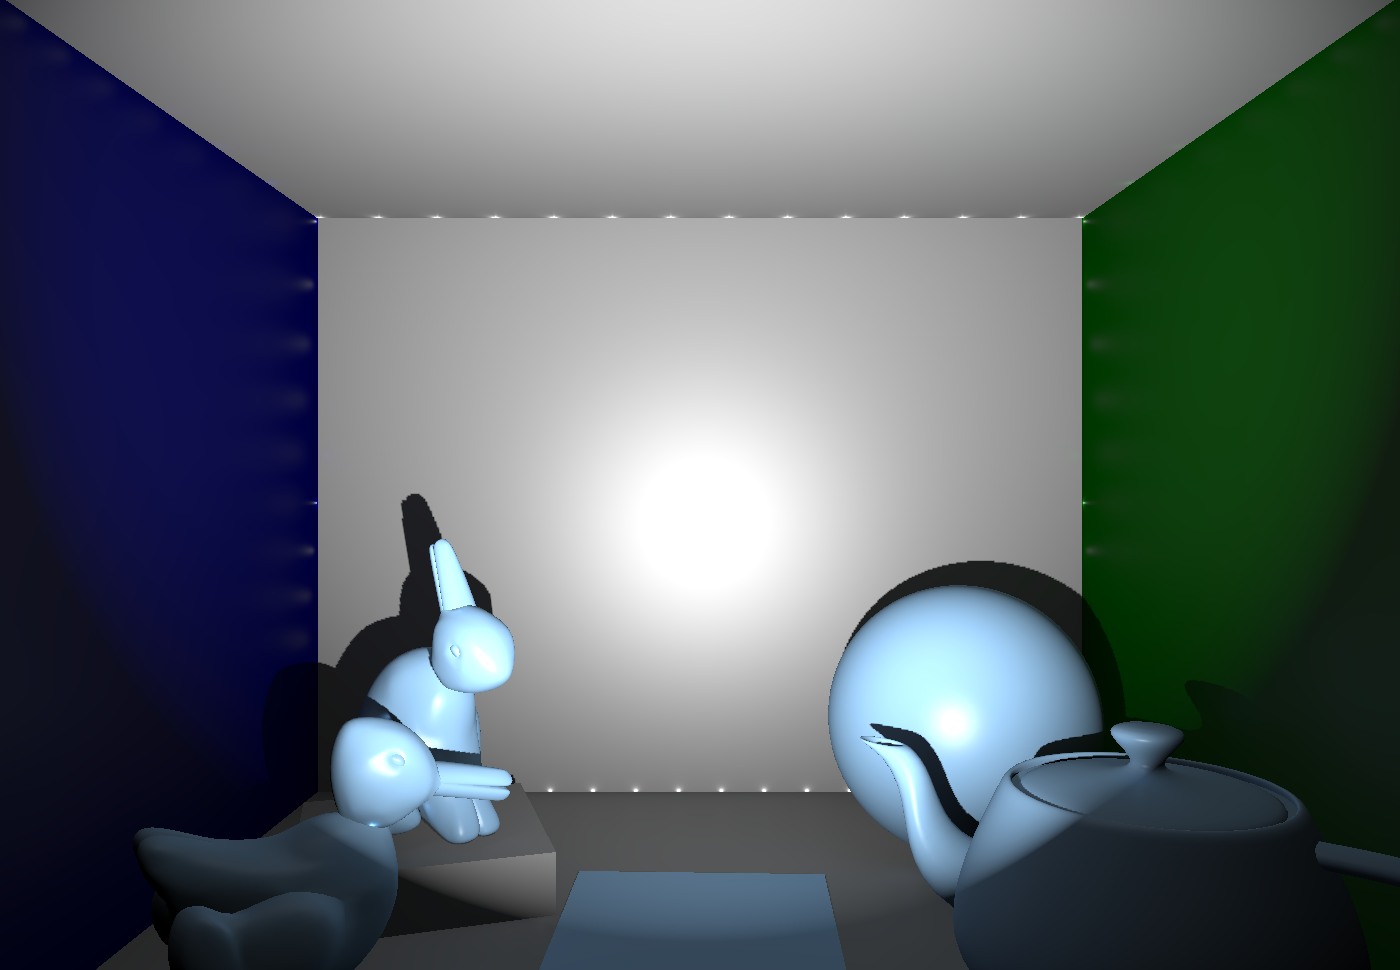
\includegraphics[width=\textwidth]{rsmbias/default}
\end{subfigure}
\begin{subfigure}[b]{0.48\textwidth}
	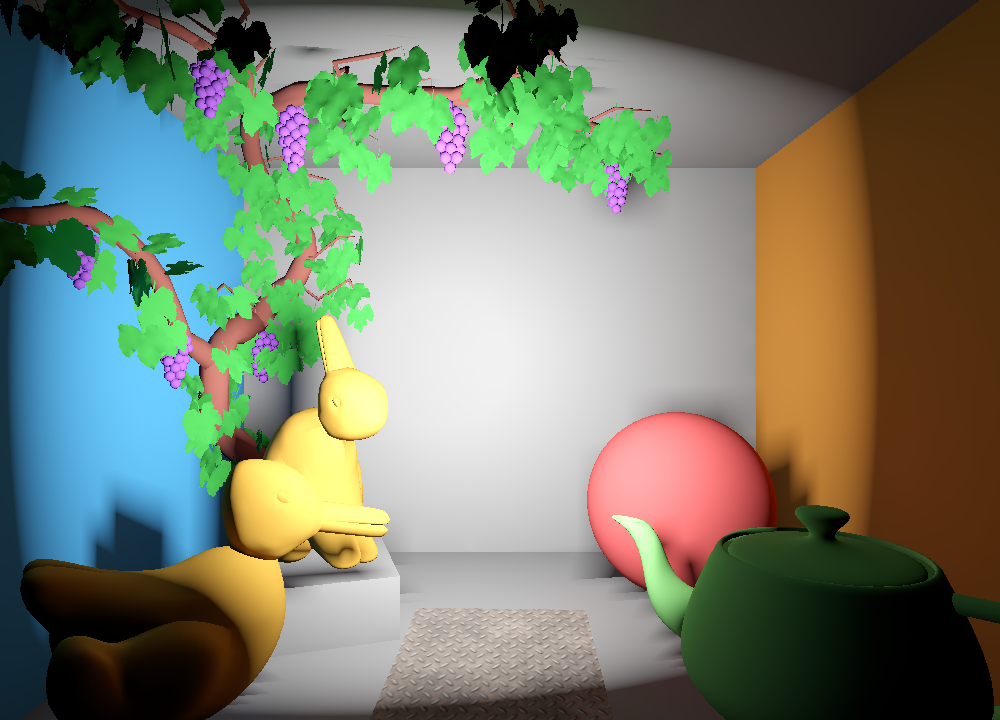
\includegraphics[width=\textwidth]{rsmbias/val}
\end{subfigure}
\caption{Left: Small bright splotches due to inverse squared distance in geometry term. Right: Using virtual area lights as proposed in \cite{bib:LightskinPaper}.}\label{fig:rsmbias}
\end{figure}
The inverse-squared distance between shading point and light source introduces a singularity, as this distance is zero in the limit.
Therefore, the contribution of a VPL reaches infinity in such a point.
The result are bright splotches, mostly visibility in creases, as seen left in \autoref{fig:rsmbias}.

Typically these artifacts are avoided by clamping the geometry term to a user defined maximum.
Obviously this introduces a bias.
There are several bias compensation techniques:
Kollig and Keller \cite{bib:biascomp:kk04} shoot rays to nearby surface and evaluate the lighting there to transport it back to the original surface.
However, this technique may degenerate to path-tracing is thus not suitable for interactive applications.
Other techniques try to compensate the bias approximately.
For example the bias compensation by Nov\'{a}k et al. \cite{bib:biascomp:novak11} stores the bounded transport in screen-space and computes then residual transport.
Although it misses invisible surfaces, it is both efficient and plausible in its results. \todo{there are more. Note more?}
\\
There are also several approaches that use different types of virtual light sources instead of VPLs.
Ha{\v{s}}an et al. \cite{bib:biascomp:vsl} introduce a new light type, the virtual spherical light (VSL).
Instead of a point-to-point evaluation, this allows them to integrate over the solid angle subtended by the spherical light sources.
Their approach is biased but does not cause bright splotches and preserves the overall energy by redistributing.
\\
Lensing et al. \cite{bib:LightskinPaper} use approximate disc shaped lights.
Since they use reflective shadow maps, the area of these virtual areal lights (VAL) $A_{VAL}$ can easily be estimated by the distance of the VAL to the light source and the solid angle a RSM texel subtends.
They show that the geometry term has an analytical solution if all surfaces are assumed to be diffuse:
\begin{align}
G(\mathrm{x}, \mathrm{x}_i)_{VAL} = \frac{(\hat{\mathbf{n}} \cdot \overrightarrow{\mathrm{x}\mathrm{x}_i} )^+}{||\mathrm{x} - \mathrm{x}_i||^2 + A_{VAL}} \cdot (\hat{\mathbf{n}}_i \cdot \overrightarrow{\mathrm{x}_i\mathrm{x}})^+
\end{align}
Using this geometry term, splotches at specular surfaces with low roughness can still occur.
However, most singularities are no longer visible (see \autoref{fig:rsmbias} right).
We use this technique in our approach since it is extremely fast, easy to implement and more plausible than a bounded geometry term.

Bias compensation in participating media are considerably more complex but not handled in this thesis.

\subsection{Shadows for Many Lights}
Book about realtime shadows (2011)\cite{bib:realtimeshadowsbook}.\\
Imperfect shadow maps Ritschel et. al. \cite{bib:imperfectshadowmaps}.\\

Virtual Shadows: Shadow Mapping using a Virtual Texturing. TODO Read, there is much more to this. \cite{bib:virtualshadowmaps}

\subsection{Shading}
Multi-resolution splatting techniques ([All Nichols] Hierarchical
image-space radiosity for interactive global illumination, Multiresolution splatting for indirect illumination, Interactive indirect illumination using adaptive multiresolution splatting) are not as efficient as "Tiled Deferred Shading" (according to \cite{bib:clusturedpreconvoledradiancecaching} (where it is just a side note!)) ... logically Tiled Deferred Shading is even better.
Interleaved Sampling (Interleaved sampling. In
Proc. of Eurographics Workshop on Rendering (2001)) also a good idea 

Clustured Forward/Deferred Shading: Finding Unique clusturs is DIFFERENT in paper \cite{bib:clusturedshading} and practical implementation like "Pratical Clustured Shading" (SIGG2013, Humus). Paper uses (local) sorting and page tables. Humus uses Volume Texture. Ollson Siggra2013 presentation uses parallel prefix sum.



\section{Discrete Ordinate Methods}
GPU Radiosity (because its the king of discrete methods!).\\
Light Propagation Volumes.\\
Voxel Cone Tracing and Voxel Based GI.\\
Radiance Hints \cite{bib:radiancehints}.


\subsection{Light Propagation Volumes}


\section{Light Caching Methods}

\subsection{(Irr-)Radiance Caching}
Irradiance Caching \cite{bib:irradiancecaching}.\\
Radiance Caching \cite{bib:radiancecaching}.\\
GPU versions


(Clustered) Preconvoled Radiance Caching \cite{bib:clusteredpreconvoledradiancecaching}
"Pre-convolved radiance caching (PCRC) [SNRS12] proposes to store incident radiance in a texture with one texel per direction and preconvolve it—in essence creating a mip-map-pyramid of the
radiance texture with accumulated radiance in the higher
levels. Additionally, a low-resolution mip-map level is cosine folded to store irradiance. Using these two textures, evaluating the RCs requires only two texture lookups instead of re-evaluating the reflection functions. Irradiance can also be gathered into screen-space caches from a photon map [WWZ09] to integrate caustics." (from \cite{bib:clusteredpreconvoledradiancecaching})\\
Improvements in the clustured algorithm: "Creation" via Voxel Cones, "Distribution" in ScreenSpace, "Evaluation" gathering instead of splatting. The "Distribution" works similar to clustured deferred shading - each cluster results in a radiance cache with an interesting way to extract the normal. Evaluation scheme is extremely simple, does not take cache normals into account. Of course no temporal coherence -.-

\subsection{Light Skin}
There is this paper \cite{bib:LightskinPaper} of Lensing et. al.


\section{Voxel Cone Tracing and Extensions}

\todo{original voxel cone tracing} Has been evaluated in game engines. "MITTRING M.: The Technology Behind the Unreal Engine 4 Elemental demo. SIGGRAPH 2012 Advances in RealTime Rendering in 3D Graphics and Games Course, 2012." 

Layered Reflective Shadow Maps for Voxel-based Indirect Illumination decouples occlusion from lighting data.
Visibility determination is handled via Voxel Cone tracing while the actual lighting is performed by lookups in a pre-filtered Layered Reflective Shadow Map.
Doing so avoids most of the memory and initialization/update overhead associated with the large voxel data structure, since each voxel encodes only binary visibility information.
Layers to avoid discontinuities, etc.

\subsection{Voxelization}

\cite{bib:GPUGems2}[Chapter 42] $http://http.developer.nvidia.com/GPUGems2/gpugems2_chapter42.html$

Modern GPU in OpenGL Insights \cite{bib:openglinsightsvoxel}

Maxwell GPUs per Hardware

\subfilebib % Makes bibliography available when compiling as subfile
\end{document}